\chapter{Validating our methodology}\label{sec:exps1}

\section{Computing Baseline Policies}

\subsection{Setup}
All the experiments presented next run on a dedicated cluster of Intel Xeon Gold 6130 (Skylake-SP), 2.10GHz, 2 CPUs/node, 16 cores/CPU with a timeout of 4 hours per experiment. Codes to reproduce our results are given in the supplementary material. In the future, we will open source a python library with all the tools of our methodology.
Using Algorithm \ref{alg:distill}, we distill deep neural network expert policies into less complex policy classes.

\paragraph{Policy classes}

\begin{table}[ht]
\centering
\small
\begin{tabular}{lll}
\hline
\textbf{Policy Class} & \textbf{Parameters} & \textbf{Training Algorithm} \\
\hline
Linear Policies & Determined by state-action dimensions & Linear/Logistic Regression \\
Decision Trees & [4, 8, 16, 64, 128] nodes & CART ($2\times$ nodes maximum leaves) \\
Oblique Decision Trees & [4, 8, 16, 64, 128] nodes & CART ($2\times$ nodes maximum leaves) \\
ReLU MLPs & [2$\times$2, 4$\times$4, 8$\times$8, 16$\times$16] weigths & Adam optimization (500 iterations) \\
\hline
\end{tabular}
\caption{Summary of baseline policy classes parameters and fitting algorithms (used in Line \ref{alg:fit}).}
\label{tab:policy-classes}
\end{table}

 We consider four policy classes for our baselines. We choose those policy classes because there exist efficient algorithms to fit them with supervised data which is a required step of imitation learning in Line \ref{alg:fit}. We consider linear policies that have been shown to be able to solve Mujoco tasks~\cite{empirical-evidence}. We fit linear policies to expert policies using simple linear (logistic) regressions with scikit-learn~\cite{scikit-learn} default implementation. We also consider decision trees~\cite{cart} and oblique decision trees~\cite{oblique}. (Oblique) Decision trees are often considered the most interpretable model class in machine learning~\cite{mythos} and reinforcement learning~\cite{viper,IBMDP,glanois-survey,milani-survey}. We train trees using the default CART~\cite{cart} implementation of scikit-learn with varying numbers of parameters (number of nodes in the tree). We also consider MLPs with ReLU activations~\cite{relunet} with varying number of parameters (total number of weights). This class of policy is often considered the least interpretable and is often used in deep reinforcement learning~\cite{deep-rl-relu1,deep-rl-relu2,deep-rl-relu3}. We train ReLU MLPs using the default scikit-learn implementation of Adam optimization~\cite{adam} with 500 iterations. The 15 baseline policy classes that we consider are summarized in Appendix \ref{tab:policy-classes}. 
\paragraph{Neural network experts}
We do not train new deep reinforcement learning agents \cite{dqn,ppo,deep-rl-relu1} but rather re-use ones available at the stables-baselines3 zoo \cite{zoo}. Depending on the environments described next, we choose neural network policies from different deep reinforcement learning agents. Some may argue that during the imitation learning, ReLU MLPs baselines may obtain better performance because they are often from the same class as the expert they imitate unlike trees. But this is not of our concern as we do not benchmark the imitation learning algorithms. Furthermore, it is important to note that not all experts are compatible with all the variants of imitation learning Algorithm \ref{alg:distill}. Indeed, SAC experts \cite{deep-rl-relu1} are not compatible with $Q$-DAgger \cite{viper} because it only works for continuous actions; and PPO experts, despite working with discrete actions do not compute a $Q$-function necessary for the re-weighting in $Q$-DAgger.

\paragraph{Environments}
We consider common environments in reinforcement learning research. We consider the classic control tasks from gymnasium \cite{gymnasium}, MuJoCo robots from \cite{mujoco}, and Atari games from \cite{atari}. For Atari games, since the state space is frame pixels that can't be interpreted, we use the object-centric version of the games from \cite{ocatari}. In Appendix \ref{tab:envs} we give the list of environments we consider in our experiments with their state-action spaces as well as a cumulative reward threshold past which an environment is consider ``solved''.

\subsection{Ablation study of imitation learning}\label{sec:res-imit}

In this section, we present the results of the expert distillation into smaller policies. For each environment, we fit all the policy classes. To do so, we run different instantiations of Algorithm \ref{alg:distill} multiple times with different total sample sizes. For each environment and each imitation learning variant, we summarize the number of times we fit all the baselines to an expert and which expert we use. The number of runs and imitation algorithm variants of Algorithm \ref{alg:distill} are summarized in Appendix \ref{tab:repet-distill}. After running the imitation learnings, we obtain roughly 40000 baseline policies (35000 for classic control, 5000 thousands for MuJoCo and 400 for OCAtari). A dataset with all the baselines measurements is given in the supplementary material.

\begin{figure}[ht]
\centering
\begin{subfigure}{.33\textwidth}
  \centering
  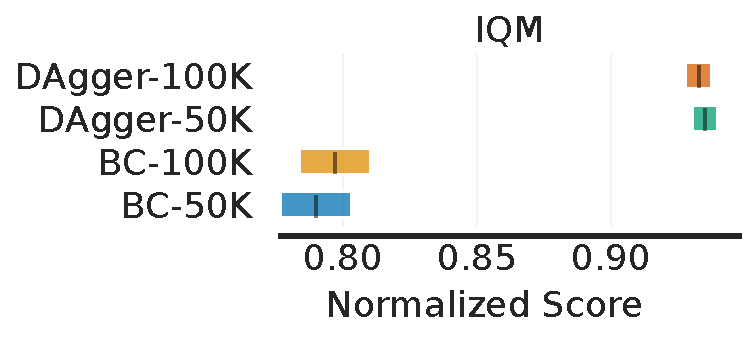
\includegraphics[width=\linewidth]{images/images_part3/ppo_expert_classic_control.pdf}
  \caption{Classic control, PPO expert}
  \label{fig:ppo_classic}
\end{subfigure}%
\begin{subfigure}{.33\textwidth}
  \centering
  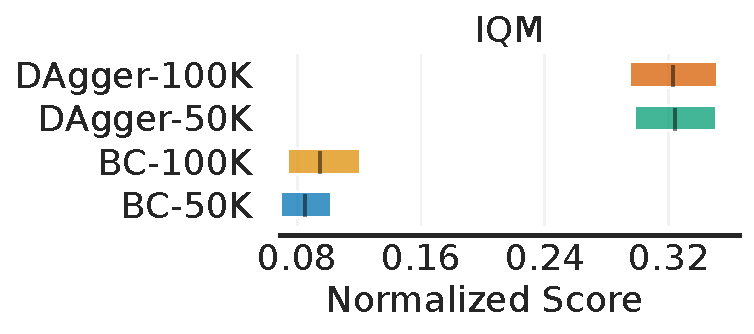
\includegraphics[width=\linewidth]{images/images_part3/sac_expert_mujoco.pdf}
  \caption{MuJoCo, SAC expert}
  \label{fig:sac_mujoco}
\end{subfigure}
\begin{subfigure}{.33\textwidth}
  \centering
  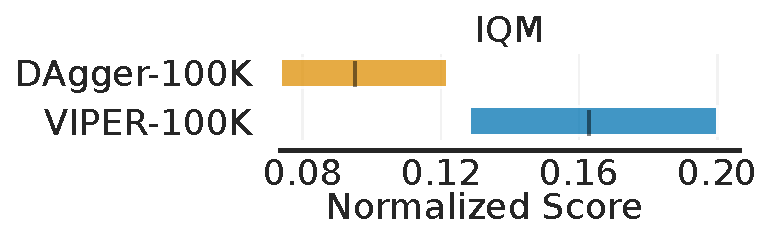
\includegraphics[width=\linewidth]{images/images_part3/dqn_expert_atari.pdf}
  \caption{OCAtari, DQN expert}
  \label{fig:dqn_atari}
\end{subfigure}%
\caption{Performance of imitation learning variants of Algorithm \ref{alg:distill} on different environments. We plot the 95\% stratified bootstrapped confidence intervals around the IQMs.}
\label{fig:performance_comparison}
\end{figure}

\paragraph{What is the best imitation algorithm?}
Even though the focus of our work is to evaluate trained policies, we still provide some insights on the best way to obtain interpretable policies from experts. Using the reinforcement learning evaluation library rliable~\cite{rliable}, we plot on Figure \ref{fig:performance_comparison} the interquartile means (IQM, an estimator of the mean robust to outliers) of the baseline policies cumulative rewards averaged over 100 episodes. For each imitation algorithm variant, we aggregate cumulative rewards over environments and policy classes. We normalize the baselines cumulative rewards between expert and random agent cumulative rewards.

The key observation is that for tested environments (Figures \ref{fig:ppo_classic},\ref{fig:sac_mujoco}), Behavior Cloning is not an efficient way to train baseline policies compared to DAgger. This is probably because Behavior Cloning trains a student policy to match the expert's actions on states visited by the expert while DAgger trains a student to take the expert's actions on the states visited by the student~\cite{dagger}. An other observation is that the best performing imitation algorithms for MuJoCo (DAgger, Figure \ref{fig:sac_mujoco}) and OCAtari ($Q$-Dagger, Figure \ref{fig:dqn_atari}) obtain baselines that in average cannot match well the performances of the experts. However baseline policies almost always match the expert on simple tasks like classic control (Figure \ref{fig:ppo_classic}).

\paragraph{What is the best policy class in terms of reward?}

\begin{figure}[ht]
    \centering
    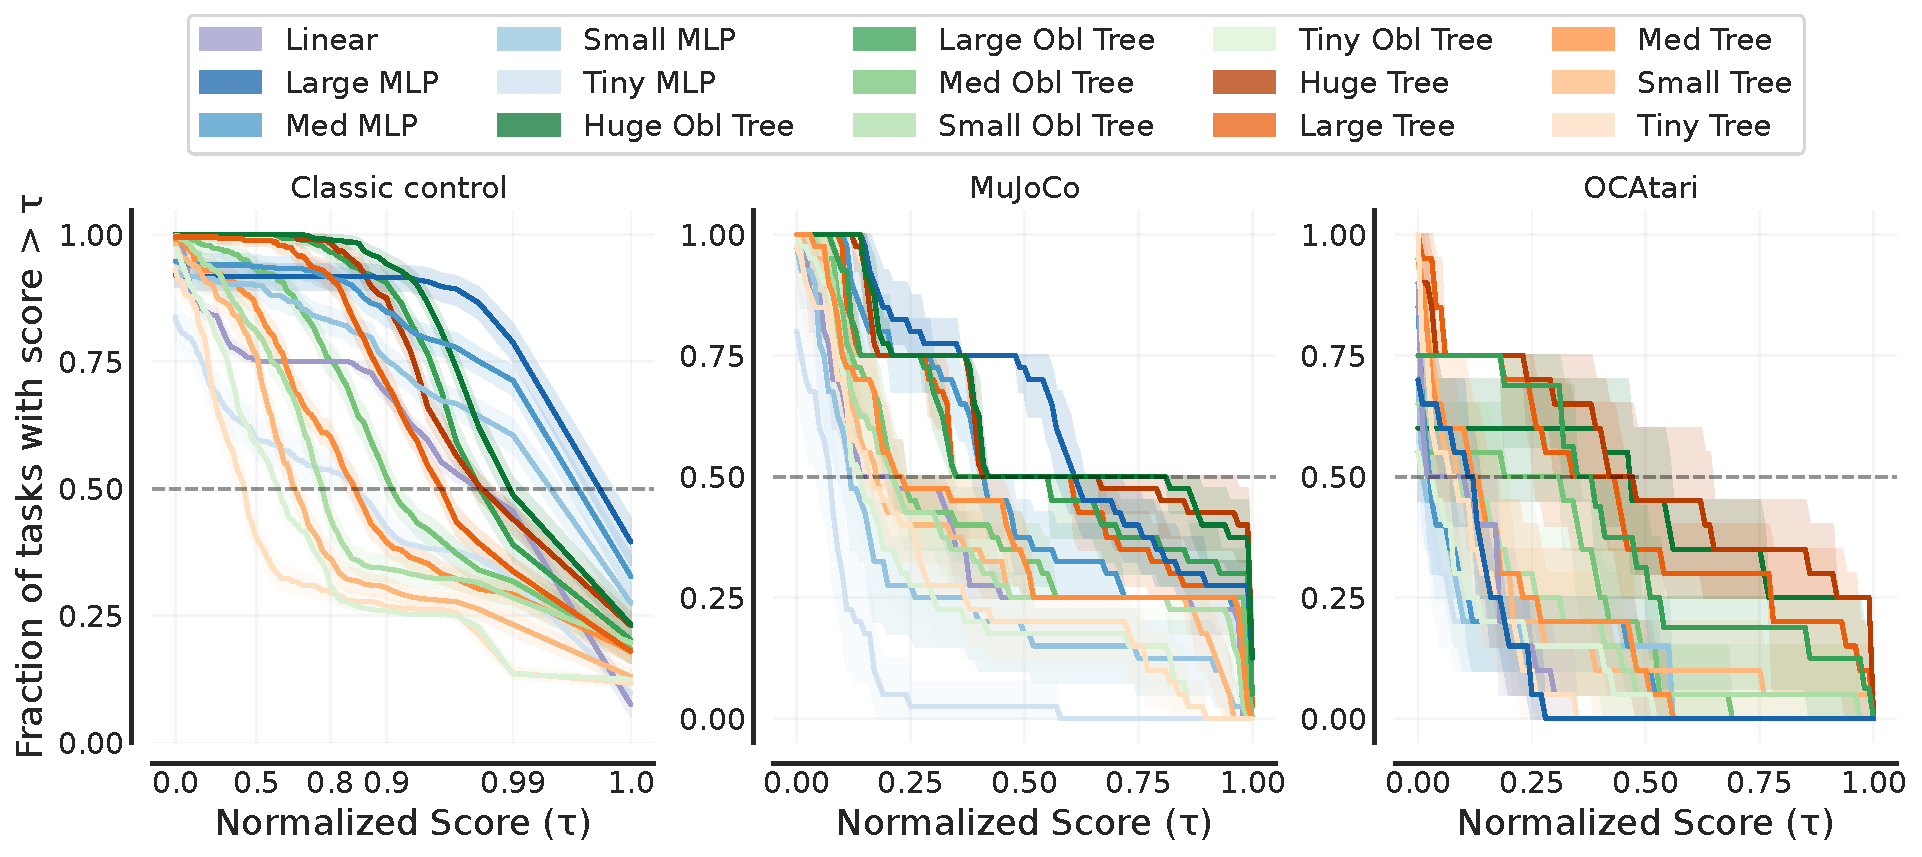
\includegraphics[trim={0 0 0 0.2cm},clip,width=0.9\linewidth]{images/images_part3/perf_profile_combined_100k.pdf}
    \caption{Performance profiles of different policy classes on different environments.}
    \label{fig:perf-combined}
\end{figure}

We also wonder if there is a policy class that matches expert performances more often than others across environments. For that we plot performance profiles of the different policy classes obtained with a fixed expert and fixed imitation learning algorithm. In particular, for each environments group we use the baseline policies obtained from the best performing imitation learning algorithm from Figure \ref{fig:performance_comparison}. From Figure \ref{fig:perf-combined} we see that on classic control environments, MLPs tend to perform better than other classes while on OCAtari games, trees tend to perform better than other classes. Now we move on to interpretability evaluation of our programmatic policies.



\section{Measuring Policy Interpretability}\label{sec:ablation-metric}
\subsection{From Policy to Program}
\begin{figure}
    \centering
    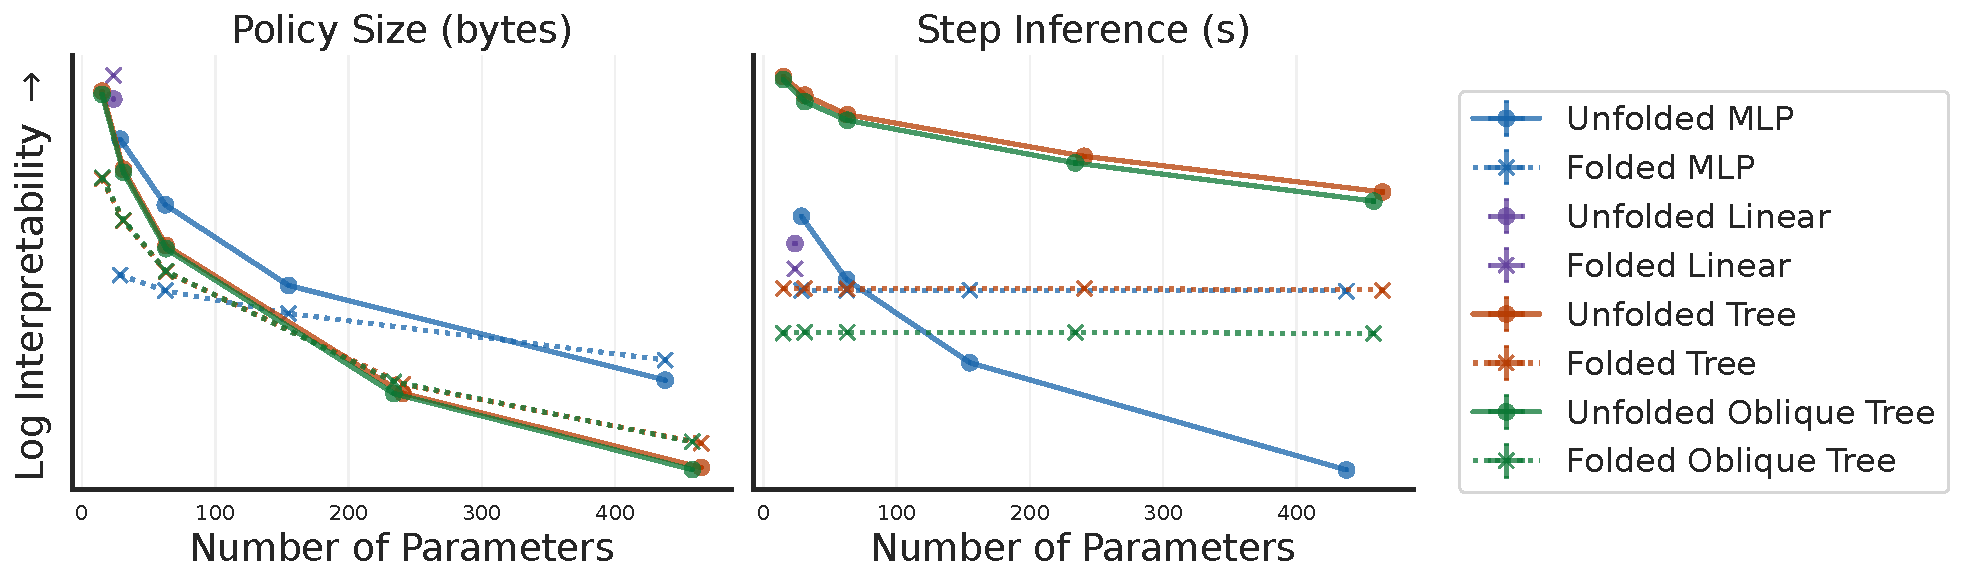
\includegraphics[width=1\linewidth]{images/images_part3/tree_sizes_memory_ppo_ci_ablation.pdf}
    \caption{Policies interpretability on classic control environments. We plot 95\% stratified bootstrapped confidence intervals around means in both axes. In each sub-plot, interpreatbility is measured with either bytes or inference speed.}
    \label{fig:abl-proxies}
\end{figure}

In this section, we compute the step inference times, as well as the policy size for both the folded and unfolded variant of each policy obtained for classic control environments with DAgger-100K. To unfold policies, we convert them into Python programs formatted with PEP 8 (comparing other unfolding formats such as ONNX \url{https://github.com/onnx/onnx} is left to future work). We ensure that all policies operations are performed sequentially and compute the metrics for each policy on 100 episodes using the same CPUs.

\paragraph{Is it necessary to unfold policies to compute interpretability metrics?} We see on Figure \ref{fig:abl-proxies} that folded policies of the same class almost always give similar interpretability values (dotted lines) despite having very different number of parameters. Hence, measuring folded policies interpretability would contradict established results from user studies such as, e.g., trees of different sizes have different levels of interpretability~\cite{study-4}. 

\paragraph{Is there a best policy class in terms of interpretability?}
User studies from~\cite{study-1,study-2,study-3} show that decision trees are easier to understand than models involving mathematical equations like oblique trees, linear maps, and MLPs. However,~\cite{mythos} states that for a human wanting to have a global idea of the inference of a policy, a compact MLP can be more interpretable than a very deep decision tree. In Figure \ref{fig:abl-proxies}, we show that inference speed and memory size of programs help us capture those nuances: policy interpretability does not only depend on the policy class but also on the metric choice. Indeed, when we measure interpretability with inference times, we do observe that trees are more interpretable than MLPs. However, when measuring interpretability with policy size, we observe that MLPs can be more interpretable than trees for similar number of parameters. Because there seem to not be a more interpretable policy class across proxy metrics, we will keep studying both metrics at the same time.
